\section{MLP vs RNN}
We will now compare the experimental results obtained by the
MLP and RNN-based models.
To do this, we will retest both networks on the testing dataset,
forcing the generation of gaps that are consistently two days
long to facilitate comparison (see Section~\ref{sec:mlpbaseline}
and Section~\ref{sec:rnnbasemodel}).
We will compare their performance by calculating, for each of them,
the pointwise error between ground truth and prediction.
Additionally, we will compare the various other metrics used
and discuss some strengths and weaknesses of each model.

%Confronteremo ora i risultati sperimentali ottenuti
%dai modelli basati su MLP e RNN. Per farlo andremo a testare nuovamente
%le due reti sul dataset di testing forzando la generazione di buchi
%sempre a 2 giorni, in modo tale da poter confrontare i risultati (vedi 
%Sezione~\ref{sec:mlpbaseline} e \ref{sec:rnnbasemodel}). Metteremo quindi
%a confronto le performance di questi andando a calcolare, per ognuno,
%l'errore puntuale tra ground truth e predizione. 
%Infine, oltre a confrontare tra di loro le altre varie metriche impiegate,
%andremo a discutere alcuni punti di forza e debolezze di ogni modello.

\begin{table}[H]
	\centering
	\begin{tabular}{l|l|l|l|l}
		\multicolumn{1}{c|}{\textbf{Gap}}       &
		\multicolumn{2}{c|}{\textbf{MAE (kW)}}  &
		\multicolumn{1}{c|}{\textbf{Diff (kW)}} &
		\multicolumn{1}{c}{\textbf{Diff (\%)}}                                                \\ %% ((MLP - RNN)*100)/MLP
		\hline
		                                        & \textit{MLP} & \textit{RNN} &       &       \\
		02-04 to 03-04                          & 18.63        & 3.91         & 14.72 & 79.01 \\
		03-04 to 04-04                          & 06.90        & 3.29         & 03.61 & 52.31 \\
		04-04 to 05-04                          & 10.41        & 5.55         & 04.86 & 46.68 \\
		05-04 to 06-06                          & 17.99        & 6.89         & 11.10 & 61.70 \\
		06-04 to 07-04                          & 20.07        & 6.78         & 13.29 & 66.21 \\
		07-04 to 08-04                          & 14.77        & 9.25         & 5.52  & 37.37 \\
		08-04 to 09-04                          & 15.82        & 7.85         & 7.97  & 50.39 \\
		09-04 to 10-04                          & 10.30        & 5.82         & 4.48  & 43.49
	\end{tabular}
	\caption{This table highlights the difference between the error of the MLP-based model and the RNN-based model. The column \texttt{Diff (kW)} represents the absolute difference between MLP MAE and RNN MAE, while \texttt{Diff (\%)} represents the percentage difference.}
	%In questa tabella viene messo in evidenza la differenza tra l'errore del modello basato su MLP e quello su Reti Ricorrenti. La colonna \texttt{Diff (kW)} è la differenza in valore assoluto tra MLP MAE e RNN MAE, mentre \texttt{Diff (\%)} è la differenza in percentuale.}
	\label{tab:mlpvsrnndiff}
\end{table}

\begin{table}[H]
	\begin{minipage}[t]{.45\textwidth}
		\centering
		\begin{tabular}[t]{l|l|l|l}
			\multicolumn{1}{c|}{\textbf{GAP}}      &
			\multicolumn{2}{c|}{\textbf{Max Err.}} &
			\multicolumn{1}{c}{\textbf{Diff.}}                                           \\
			\hline
			                                       & \textit{MLP} & \textit{RNN} &       \\
			02-04 to 03-04                         & 90.74        & 35.74        & 55.0  \\
			03-04 to 04-04                         & 96.29        & 21.69        & 74.60 \\
			04-04 to 05-04                         & 89.01        & 54.95        & 26.06 \\
			05-04 to 06-06                         & 105.01       & 53.91        & 51.10 \\
			06-04 to 07-04                         & 122.56       & 51.35        & 71.21 \\
			07-04 to 08-04                         & 105.94       & 75.91        & 30.03 \\
			08-04 to 09-04                         & 86.14        & 75.47        & 05.65 \\
			09-04 to 10-04                         & 78.76        & 59.97        & 18.79
		\end{tabular}
		\caption*{(a)}
		%\caption{Nella tabella viene mostrata la differenza tra i valori dell'indice $R^2$ per i due modelli.}
	\end{minipage}%
	\hfill
	\begin{minipage}[t]{.45\textwidth}
		\centering
		\begin{tabular}[t]{l|l|l|l}
			\multicolumn{1}{c|}{\textbf{GAP}}      &
			\multicolumn{2}{c|}{\textbf{Min Err.}} &
			\multicolumn{1}{c}{\textbf{Diff.}}                                           \\
			\hline
			                                       & \textit{MLP} & \textit{RNN} &       \\
			02-04 to 03-04                         & 7.58         & 0.90         & 6.68  \\
			03-04 to 04-04                         & 0.79         & 0.05         & 0.74  \\
			04-04 to 05-04                         & 0.39         & 0.85         & -0.46 \\
			05-04 to 06-06                         & 1.45         & 0.05         & 1.40  \\
			06-04 to 07-04                         & 4.84         & 0.13         & 4.71  \\
			07-04 to 08-04                         & 1.73         & 1.39         & 0.34  \\
			08-04 to 09-04                         & 5.19         & 0.89         & 4.30  \\
			09-04 to 10-04                         & 3.19         & 0.71         & 2.48
		\end{tabular}
		\caption*{(b)}
	\end{minipage}
	\begin{minipage}{\textwidth}
		\centering
		\begin{tabular}[t]{l|l|l|l}
			\multicolumn{1}{c|}{\textbf{GAP}}   &
			\multicolumn{2}{c|}{\textbf{$R^2$}} &
			\multicolumn{1}{c}{\textbf{Diff.}}                                        \\
			\hline
			                                    & \textit{MLP} & \textit{RNN} &       \\
			02-04 to 03-04                      & 0.64         & 0.98         & -0.34 \\
			03-04 to 04-04                      & 0.52         & 0.91         & -0.39 \\
			04-04 to 05-04                      & 0.52         & 0.89         & -0.37 \\
			05-04 to 06-06                      & 0.42         & 0.91         & -0.49 \\
			06-04 to 07-04                      & 0.62         & 0.95         & -0.33 \\
			07-04 to 08-04                      & 0.78         & 0.91         & -0.13 \\
			08-04 to 09-04                      & 0.55         & 0.85         & -0.30 \\
			09-04 to 10-04                      & 0.42         & 0.78         & -0.36
		\end{tabular}
		\caption*{(c)}
	\end{minipage}

	\caption{The tables compare the results of the two models, highlighting the maximum pointwise error (a) expressed in kW, the minimum pointwise error (b) expressed in kW, and the $R^2$ index (c). For each metric, the difference between the two values ($MPL - RNN$) is also shown.}
	%Le tabelle mettono a confronto i risultati dei due modelli paragonando il massimo errore puntuale (a) espresso in kW, il minimo errore puntuale (b) espresso in kW e l'indice $R^2$ (c). Per ognuna viene mostrata anche la differenza tra i due valore ($MPL - RNN$).}
\end{table}

From the previous tables, it's evident that the RNN-based model achieves significantly higher $R^2$ values compared to the MLP-based model. On average, the RNN-based model's values hover around 0.90, while the MLP-based model is around 0.60, with an average difference of 0.30 points. The second model approximates the trend of instant energy production during gaps much better.

In tables (a) and (b), it can be observed that the architecture utilizing RNN has maximum and minimum error values significantly lower than the MLP-based model.

Regarding Gap MAE, the second model is also superior to the first by approximately 60\%, with significantly lower average errors.

%Dalle precedenti tabelle possiamo vedere com il modello basato su RNN ottiene
%predizioni con un indice $R^2$ molto superiore a quello del modello basato su MLP. In media i valori del primo si aggirano intorno a 0.90 mentre per 
%il secondo siamo sul 0.60 con una differenza media di 0.30 punti. Il secondo modello approssima nettamente meglio l'andamento dell'energia istantanea prodotta durante i buchi. 
%Dalle tabelle (a) e (b) si vede come l'architettura che sfrutta RNN 
%ha valori di errore massimi e minimi decisamente più contenuti rispetto a quella che
%si basa su MLP.
%Anche per il Gap MAE possiamo vedere come il secodo modello
%sia migliore rispetto al primo di circa il 60\% commettendo in media errori
%nettamente più bassi rispetto all'altro.

\begin{figure}[H]
	\centering
	\begin{subfigure}{\textwidth}
		\centering
		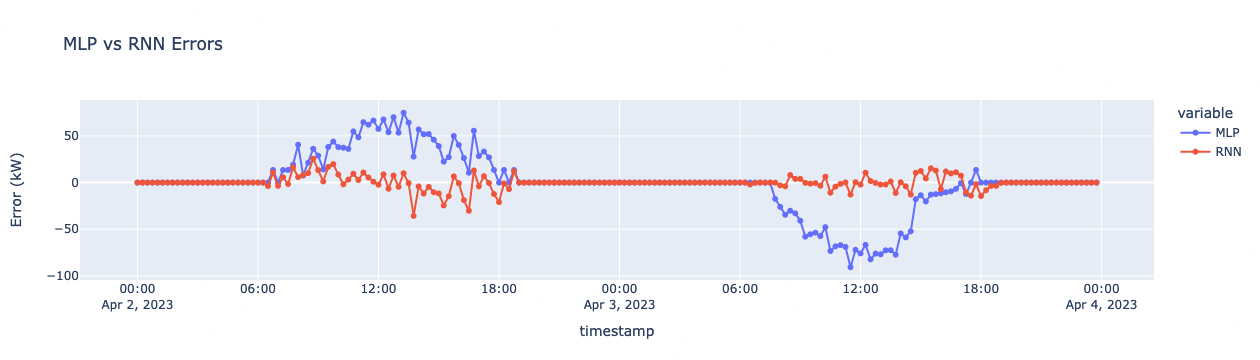
\includegraphics[width=\textwidth]{chapters/4_evaluation/imgs/mlpvsrnn/mlpvsrnn1.png}
		\caption{}
	\end{subfigure}
	\begin{subfigure}{\textwidth}
		\centering
		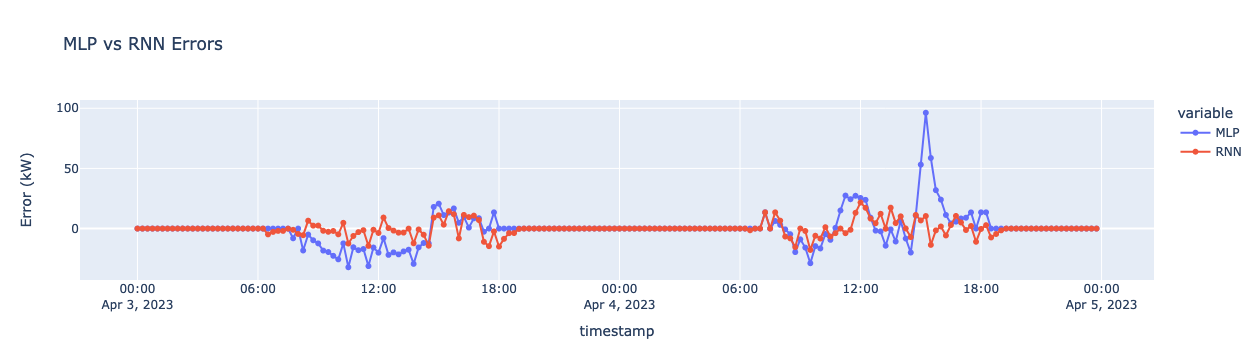
\includegraphics[width=\textwidth]{chapters/4_evaluation/imgs/mlpvsrnn/mlpvsrnn2.png}
		\caption{}
	\end{subfigure}
	\begin{subfigure}{\textwidth}
		\centering
		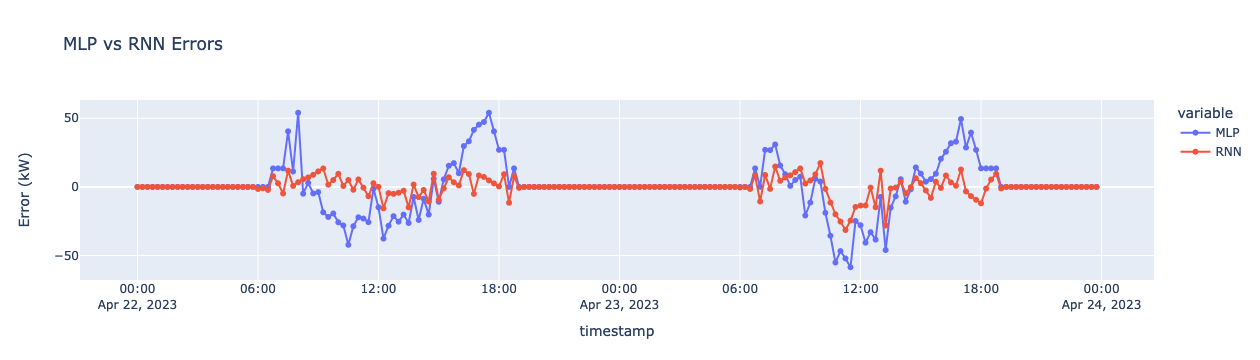
\includegraphics[width=\textwidth]{chapters/4_evaluation/imgs/mlpvsrnn/mlpvsrnn3.png}
		\caption{}
	\end{subfigure}
	\caption{The figure displays the difference curves between the target and prediction for the MLP-based models (in blue) and the RNN-based models (in red).}
	% Nella figura sono mostrate le curve delle differenze tra target e predizione dei modelli basati su MLP (mostrate in blu) e su RNN (in rosso).}
	\label{fig:mlpvsrnngrafici}
\end{figure}
From the graphs shown in Figure~\ref{fig:mlpvsrnngrafici},
it's immediately noticeable that the architecture utilizing
recurrent neural networks commits significantly lower errors
than the MLP-based model.
The red curves are generally more compact and closer to 0
(no error committed), while the blue curves are on average
much farther from the ideal value, indicating a significantly
higher pointwise error, on average by 60\%, with the presence
of substantial peaks (b).
It's important to highlight that both models do not commit errors at night.

Comparing the respective outputs of the two models,
it's evident that the predicted curves by the MLP-based model
are extremely similar to each other and fail to identify
possible production peaks.
On the other hand, the output of the second model
performs significantly better in the task, generating curves
that closely follow the ground truth, understanding the
presence of potential energy peaks, and demonstrating the
ability to generate curves with different shapes and widely
varying values.

It's also noticeable that the first model struggles with
identifying day and night periods, often ending production a
few hours before sunset.
In contrast, the second model excels in understanding
this alternation and does not exhibit issues of this nature.

It's also important to note that both models are relatively
lightweight in terms of resources for training and inference
on the architecture at our disposal.
This suggests the possibility of training and using
them on less powerful machines.

The second model can also close gaps of considerably larger
sizes than those used during the training phase.
In contrast, the first model can only handle 2-day gaps,
and to increase this limit, the model would need to repeat
the training phase.

%Dai grafici mostrati in Figura~\ref{fig:mlpvsrnngrafici} possiamo 
%notare immediatamente che l'architettura che sfrutta le reti ricorrenti
%commette errori significativamente più bassi di quella basata su MLP.
%Notiamo come le curve in rosso sono generalmente più compatte ed abbastanza
%vicine allo 0 (nessun errore commesso). Mentre quelle in blu risultano mediamente
%molto più distanti dal valore ideale evidenziando quindi un errore puntuale nettamente più alto, in media del 60\%, con la presenza di picchi di notevole valore (b). \'{E} importante evidenziare che di notte tutti e
%due i modelli non commettono errori.

%Confrontando i relativi output dei due modelli possiamo notare come
%le curve predette dal modello basato su MLP siano estremamente simili
%tra di loro e non riescono ad individuare possibili picchi di produzione.
%Mentre l'output del secondo riesce nettamente meglio nel compito generando
%curve che seguno bene l'andamento della ground trouth, riuscendo a comprendere
%anche presenza di possibili picchi di energia prodotta oltre all'abilità
%di generare curve di differente forma e valori anche moltro diversi
%tra di loro.

%Notiamo anche che il primo modello ha qualche difficoltà nel capire 
%i periodi di giorno e notte con il risultato che molto spesso termina la 
%produzione qualche ora prima del tramonto, mentre il secondo riesce molto
%bene a comprendere questa alternanza e non presenta probemi di questo tipo.

%\'{E} importante anche notare che tutti e due i modelli risultano relativamente
%leggeri sia in termini di risorse per l'allenamento e per l'inferenza sull'architettura a nostra disposizione. Suggerendo quindi la possibilità
%di essere addestrati ed usati anche su macchine meno performanti.

%Il secondo modello riesce anche a chiudere buchi di dimensioni notevolmente
%maggiori rispetto a quelli utilizzati durante la fase di training, mentre il primo riesce a gestire solo buchi di 2 giorni e per poter aumentare questo limite, il modello necessita di ripetere nuovamente la fase di trianing.

\begin{figure}[H]
	\centering
	\begin{subfigure}{\textwidth}
		\centering
		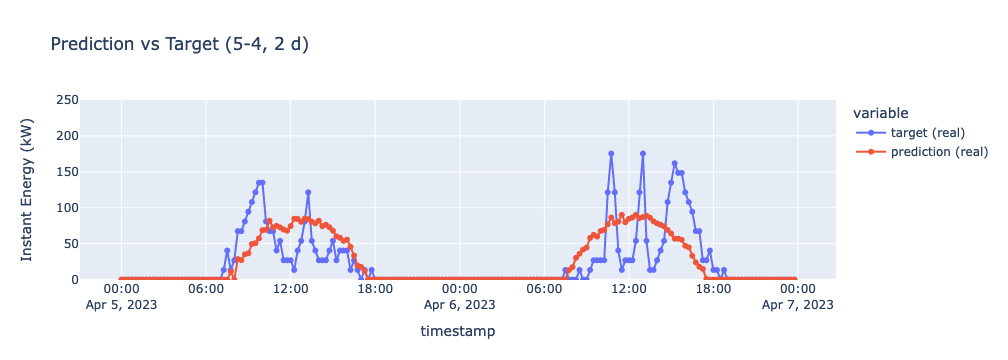
\includegraphics[width=.75\textwidth]{chapters/3_models/imgs/ufnc/eval/ufcpred5-4.png}
		\caption{}
	\end{subfigure}
	\begin{subfigure}{\textwidth}
		\centering
		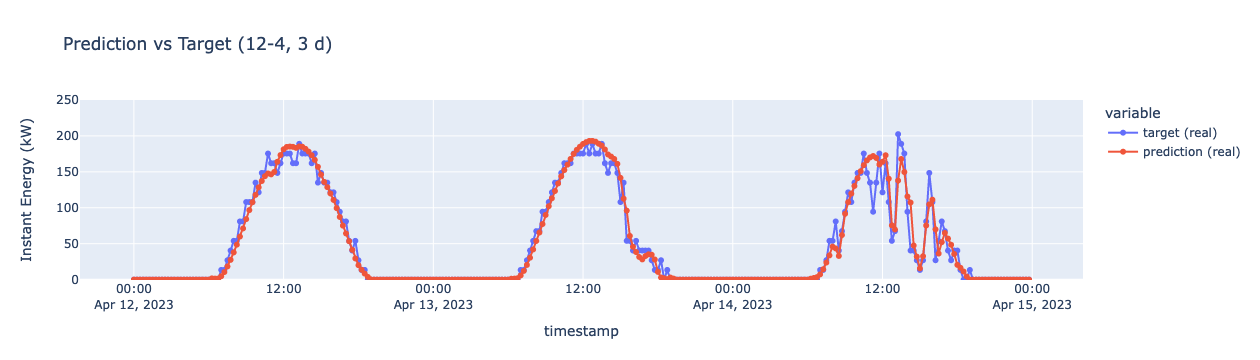
\includegraphics[width=.75\textwidth]{chapters/3_models/imgs/grrun/eval/grruneval124.png}
		\caption{}
	\end{subfigure}
	\caption{Visual comparison between an output of the MLP-based model (a) and an output of the RNN-based model (b).}
	%Confronto visuale tra un output del modello basato su MLP (a) e output del modello basato su RNN (b).}
\end{figure}
